\documentclass{bioinfo}
\copyrightyear{2015}
\pubyear{2015}

\usepackage{amsmath}
\usepackage[ruled,vlined]{algorithm2e}
\newcommand\mycommfont[1]{\footnotesize\rmfamily{\it #1}}
\SetCommentSty{mycommfont}
\SetKwComment{Comment}{$\triangleright$\ }{}

\usepackage{natbib}

\bibliographystyle{apalike}

\begin{document}
\firstpage{1}

\title[Long-read mapping and assembly]{Minimap and miniasm: fast mapping and de novo assembly for noisy long sequences}
\author[Li]{Heng Li}
\address{Broad Institute, 75 Ames Street, Cambridge, MA 02142, USA}
\maketitle

\begin{methods}

\section{Methods}

\subsection{General notations}

Let $\Sigma=\{\mathrm{A},\mathrm{C},\mathrm{G},\mathrm{T}\}$ be the
alphabet of nucleotides. If symbol $a\in\Sigma$, $\overline{a}$ is the
Watson-Crick complement of $a$. For a string $s=a_1a_2\cdots a_n$ over
$\Sigma$, which is also called a \emph{DNA sequence}, its length is $|s|=n$;
its \emph{reverse complement} is $\overline{s}=\overline{a_1a_2\cdots
a_n}=\overline{a}_n\overline{a}_{n-1}\cdots\overline{a}_1$.
For convenience, we define strand function
$\pi:\Sigma^*\times\{0,1\}\to\Sigma^*$ such that $\pi(s,0)=s$ and
$\pi(s,1)=\overline{s}$.

By convention, we call a $k$-long DNA sequence as a $k$-mer. We use the
notation $s^k_i=a_i\cdots a_{i+k-1}$ to denote a $k$-long substring of $s$
starting at $i$.

\subsection{Minimap}

\subsubsection{Overview of algorithm}

Loosely speaking, a $(w,k)$-minimizer \citep{Roberts:2004fv} of a string is the
smallest $k$-mer in a surrounding window of $w$ consecutive $k$-mers. If
sequence $s'$ is a subsequence of $s$, the minimizers of $s'$ will be a subset
of the minimizers of $s$. If $s'$ and $s$ are close, the number of shared
colinear minimizers between them approximately measures their similarity. In
this sense, the set of minimizers of $s$ is a (possibly reduced) representation
of $s$. When we map a query sequence against a set of target sequences, we may
construct a hash table for all target minimizers and then look up for query
minimizers. Large clusters of colinear minimizer matches imply potential
mappings.

%A similar and more popular concept is $(w,k)$-mer, which is used by many
%aligners such as BLAT and SSAHA2. A $(w,k)$-mer of a string $s$ is a $k$-mer
%starting at position $iw$, $i\le\lfloor(|s|-k+1)/w\rfloor$. If we construct a
%hash table for all $(w,k)$-mers of target sequences, we need to look up for
%every query $k$-mer, not just the $(w,k)$-mers of the query -- in contrast, if
%we use minimizers, we only look up for query minimizers, not every $k$-mer.
%Minimizer-based mapping tends to be more efficient.

\subsubsection{Computing minimizers}

\begin{algorithm}[ht]
\DontPrintSemicolon
\footnotesize
\KwIn{Parameter $w$ and $k$ and sequence $s$ with $|s|\ge w+k-1$}
\KwOut{($w$,$k$)-minimizers, their positions and strands}
\BlankLine
\textbf{Function} {\sc MinizerSketch}$(s,w,k)$
\Begin {
	$\mathcal{M}\gets\emptyset$\Comment*[r]{NB: $M$ is a set; no duplicates}
	\For{$i\gets1$ \KwTo $|s|-w-k+1$} {
		$m\gets\infty$\;
		\nl\For (\Comment*[f]{Find the min value}) {$j\gets0$ \KwTo $w-1$} {
			$(u,v)\gets(\phi(s^k_{i+j}),\phi(\overline{s}^k_{i+j}))$\;
			\If (\Comment*[f]{Skip if strand ambiguous}) {$u\not=v$} { 
				$m\gets\min(m,\min(u,v))$\;
			}
		}
		\nl\For (\Comment*[f]{Collect minimizers}) {$j\gets0$ \KwTo $w-1$} {
			$(u,v)\gets(\phi(s^k_{i+j}),\phi(\overline{s}^k_{i+j}))$\;
			\uIf{$u<v$ {\bf and} $u=m$} {
				$\mathcal{M}\gets\mathcal{M}\cup\{(m,i+j,0)\}$\;
			}\ElseIf{$v<u$ {\bf and} $v=m$}{
				$\mathcal{M}\gets\mathcal{M}\cup\{(m,i+j,1)\}$\;
			}
		}
	}
	\Return $M$\;
}
\caption{Compute minimizers}
\end{algorithm}

Let $\phi:\Sigma^k\to\mathbb{Z}$ be a function that maps any $k$-mer to an integer.
Formally, a double-strand $(w,k,\phi)$-minimizer, or simply a minimizer, of a
string $s$, $|s|\ge w+k-1$, is a triple $(h,i,r)$ such that there exists
$\max(1,i-w+1)\le j\le\min(i,|s|-w-k+1)$ which makes
$$
h=\phi(\pi(s_i^k,r))=\min\big\{\phi(\pi(s_{j+p}^k,r')):0\le p<w,r'\in\{0,1\}\big\}
$$
Let $\mathcal{M}(s)$ be the set of minimizers of $s$.  Algorithm~1 gives the
pseudocode to compute $\mathcal{M}(s)$ in $O(w\cdot|s|)$ time.  Our actual
implementation is close to $O(|s|)$ in average case. It uses a queue to cache
the previous minimals and avoids the loops at line~1 and~2 most of time. In
practice, time spent on collecting minimizers is insignificant.

A natural choice of $\phi$ is to let $\phi(\mathrm{A})=0$,
$\phi(\mathrm{C})=1$, $\phi(\mathrm{G})=2$ and $\phi(\mathrm{T})=3$ and for a
$k$-mer $s=a_1\cdots a_k$, define
$$
\phi(s)=\phi(a_1)\times4^{k-1}+\phi(a_2)\times4^{k-2}+\cdots+\phi(a_k)
$$
It always maps a $k$-mer to a distinct integer. A problem with this function is
that ploy-A, which is often highly enriched in genomes, always gets zero, the
smallest value. The function may oversample these non-informative poly-A and
hurts practical performance. To alleviate this issue, we use $\phi'=h\circ\phi$
instead, where $h$ is an invertible integer hash function on $[0,4^k)$ as is
implemented with Algorithm~2 (http://bit.ly/invihgi). The invertibility of $h$
is not critical to the computation of minimizers, but as such $\phi'$ never
maps two distinct $k$-mers to the same $2k$-bit integer, it helps to reduce
hash collisions.

\begin{algorithm}[ht]
\DontPrintSemicolon
\footnotesize
\KwIn{$p$-bit integer $x$}
\KwOut{hashed $p$-bit integer}
\BlankLine
\textbf{Function} {\sc InvertibleHash}$(x,p)$
\Begin {
	$m\gets2^p-1$\;
	$x\gets(\mbox{\tt\char126}x+(x\mbox{\tt\char60\char60}21))\mbox{ \tt\char38}\mbox{ }m$\;
	$x\gets x\mbox{ \tt\char94}\mbox{ }x\mbox{\tt\char62\char62}24$\;
	$x\gets(x+(x\mbox{\tt\char60\char60}3)+(x\mbox{\tt\char60\char60}8))\mbox{ \tt\char38}\mbox{ }m$\;
	$x\gets x\mbox{ \tt\char94}\mbox{ }x\mbox{\tt\char62\char62}14$\;
	$x\gets(x+(x\mbox{\tt\char60\char60}2)+(x\mbox{\tt\char60\char60}4))\mbox{ \tt\char38}\mbox{ }m$\;
	$x\gets x\mbox{ \tt\char94}\mbox{ }x\mbox{\tt\char62\char62}28$\;
	$x\gets(x+(x\mbox{\tt\char60\char60}31))\mbox{ \tt\char38}\mbox{ }m$\;
	\Return $x$\;
}
\caption{Invertible integer hash function}
\end{algorithm}

Note that in a window of $w$ consecutive $k$-mers, there may be more than one
minimizers. Algorithm~1 keeps them all with the loop at line~2. This makes a
minimizer of $s$ always correspond to a minimizer of $\overline{s}$.
\citet{Roberts:2004fv} did not discuss the treatment of such equally good
minimizers.

\subsubsection{Indexing}

\begin{algorithm}[ht]
\DontPrintSemicolon
\footnotesize
\KwIn{Set of target sequences $\mathcal{T}=\{s_1,\ldots,s_T\}$}
\KwOut{Minimizer hash table $\mathcal{H}$}
\BlankLine
\textbf{Function} {\sc Index}$(\mathcal{T},w,k)$
\Begin {
	$\mathcal{H}\gets$ empty hash table\;
	\For{$t\gets1$ \KwTo $T$} {
		$\mathcal{M}\gets${\sc MinizerSketch}$(s_t,w,k)$\;
		\ForEach{$(h,i,r)\in \mathcal{M}$} {
			$\mathcal{H}[h]\gets\mathcal{H}[h]\cup\{(t,i,r)\}$\;
		}
	}
	\Return $\mathcal{H}$\;
}
\caption{Index target sequences}
\end{algorithm}

Algorithm~3 describes target indexing. It keeps minimizers in all target
sequences in a hash table where the key is the minimizer hash and the value is
a set of target sequence index, the position of the minimizer and the strand
(packed into one 64-bit integer).

In implementation, we do not directly insert minimizers to the hash table.
Instead, we append minimizers to an array and sort the array after collecting
all minimizers. The hash table keeps the intervals on the sorted array. This
procedure dramatically reduces heap allocations and cache misses, and is
supposedly faster than direct hash table insertion.

\subsubsection{Mapping}

Given two sequences $s$ and $s'$, we say we find a \emph{minimizer hit}
$(h,x,i,i')$ if there exist $(h,i,r)\in\mathcal{M}(s)$ and
$(h,i',r')\in\mathcal{M}(s')$ with $x=r\oplus r'$ ($\oplus$ is the XOR
operator). Here $h$ is the minimizer hash value, $x$ indicates the relative
strand and $i$ and $i'$ are the positions on the two sequences, respectively.
We say two minimizer hits $(h_1,x,i_1,i'_1)$ and $(h_2,x,i_2,i'_2)$ are
\emph{$\epsilon$-away} if 1) $x=0$ and $|(i_1-i'_1)-(i_2-i'_2)|<\epsilon$
or 2) $x=1$ and $|(i_1+i'_1)-(i_2+i'_2)|<\epsilon$. Intuitively,
$\epsilon$-away hits are approximately colinear within a band of width
$\epsilon$.  Given a set of minimizer hits $\{(h,x,i,i')\}$, we can cluster
$i-i'$ for $x=0$ or $i+i'$ for $x=1$ to identify long colinear matches.

\begin{algorithm}[ht]
\DontPrintSemicolon
\footnotesize
\KwIn{Hash table $\mathcal{H}$ and query sequence $q$}
\KwOut{Print matching query and target intervals}
\BlankLine
\textbf{Function} {\sc Map}$(\mathcal{H},q,w,k,g)$
\Begin {
	$\mathcal{A}\gets$ empty array\;
	$\mathcal{M}\gets${\sc MinizerSketch}$(q,w,k)$\;
	\nl\ForEach (\Comment*[f]{Collect minimizer hits}) {$(h,i,r)\in \mathcal{M}$} {
		\ForEach{$(t,i',r')\in \mathcal{H}[h]$} {
			\uIf (\Comment*[f]{Minimizers on the same strand}) {$r=r'$} {
				Append $(t,0,i-i',i')$ to $\mathcal{A}$\;
			} \Else (\Comment*[f]{On different strands}) {
				Append $(t,1,i+i',i')$ to $\mathcal{A}$\;
			}
		}
	}
	Sort $\mathcal{A}=[(t,r,c,i')]$ in the order of the four values in tuples\;
	$b\gets1$\;
	\nl\For (\Comment*[f]{Cluster minimizer hits}) {$e=1$ \KwTo $|\mathcal{A}|$} {
		\If{$e=|\mathcal{A}|$ {\bf or} $\mathcal{A}[e+1].t\not=\mathcal{A}[e].t$ {\bf or} $\mathcal{A}[e+1].r\not=\mathcal{A}[e].r$ {\bf or} $\mathcal{A}[e+1].c-\mathcal{A}[e].c>g$} {
			\nl$\mathcal{C}\gets$ the maximal colinear subset of $\mathcal{A}[b..e]$\;
			Print the left- and right-most query/target positions in $\mathcal{C}$\;
			$b\gets e+1$\;
		}
	}
}
\caption{Map a query sequence}
\end{algorithm}

Algorithm~4 gives the details of the mapping algorithm. The loop at line~1
collects minimizer hits between the query and all the target sequences. The
loop at line~2 performs a single-linkage clustering to group approximately
colinear hits. Some hits in a cluster may not be colinear because two minimizer
hits within distance $\epsilon$ are always $\epsilon$-away. To fix this issue,
line~3 finds the maximal colinear subset of hits by solving a longest
increasing sequencing problem. This subset is the final mapping result. In
practical implementation, we set thresholds on the size of the subset and the
number of matching bases in the subset to filter poor mappings.

\subsection{Assembly graph}

Two strings $v$ and $w$ may be mapped to each other based on their sequence
similarity. If $v$ can be mapped to a substring of $w$, we say $w$
\emph{contains} $v$. If a suffix of $v$ and a prefix of $w$ can be mapped to
each other, we say $v$ \emph{overlaps} $w$, or written as $v\to w$.
If we regard strings $v$ and $w$ as vertices, the overlap relationship defines
a directed edge between them. The \emph{length} of $v\to w$ equals the length
of $v$'s prefix that does not overlap $w$.

Let $G=(V,E,\ell)$ be a simple graph (i.e. no multi-edges or loops), where $V$ is a
set of DNA sequences (vertices), $E$ a set of overlaps between them (edges) and
$\ell:E\to\Re_+$ is the edge length fuction. $G$ is said to be
\emph{Watson-Crick complete} if i) $\forall v\in V$, $\overline{v}\in V$ and
ii) $\forall v\to w\in E$, $\overline{w}\to\overline{v}\in E$. $G$ is said to
be \emph{containment-free} if any sequence $v$ is not contained in other
sequences in $V$. If $G$ is both Watson-Crick complete and containment-free, it
is an \emph{assembly graph}. Let $\mathrm{deg}^+(v)$ be the indegree of $v$ and
$\mathrm{deg}^-(v)$ be the outdegree. It follows that
$\mathrm{deg}^-(v)=\mathrm{deg}^+(\overline{v})$.

An assembly graph has the same topology as a string graph~\citep{Myers:2005bh},
though the interpretation of the vertex set $V$ is different. In a string
graph, $V$ is the set of the two ends of sequences, not the set of forward and
reverse-complemented sequences.

In an assembly graph, an edge $v\to w$ is \emph{transitive} if there exist
$v\to u$ and $u\to w$. Removing a transitive edge does not affect the
connectivity of the graph. A vertex $v$ is a \emph{tip} if ${\rm deg}^+(v)=0$
and ${\rm deg}^-(v)>0$. The majority of tips are caused by artifacts or missing
overlaps. A \emph{bubble} is a directed acyclic subgraph with a single source
$v$ and a single sink $w$ having at least two paths between $v$ and $w$. The
bubble is tight if ${\rm deg}^+(v)>1$ and ${\rm deg}^-(w)>1$. A bubble may be
caused by variants between homologous haplotypes as well as missing overlaps.

\subsection{Miniasm}

\subsubsection{Trimming reads}

Raw read sequences may contain artifacts such as untrimmed adapters and
chimaera. The first step of assembly to reduce such artifacts by examining
read-to-read mappings. For each read, miniasm finds the longest region that is
covered by three or more good mappings (longer than 2000bp with at least 100bp
non-redundant bases on matching minimizers) and trims bases outside the region.
It uses the good mappings to get a very crude estiamte of sequencing coverage.
If the coverage is more than 20-fold, miniasm applies the previous filtering
strategy again but requiring reads to be covered by more good mappings (by
default, 15\% of estiamted coverage). While trimming reads, miniasm also trims
mappings.

\subsubsection{Generating assembly graph}

\begin{figure}[ht]
\centering
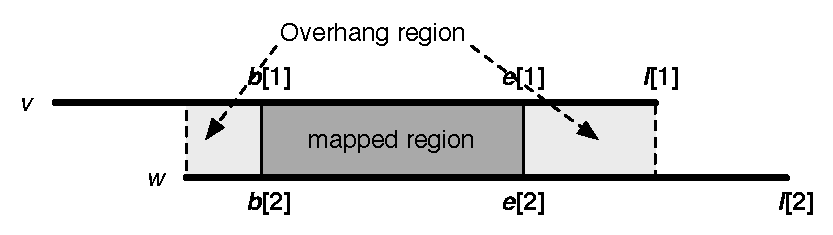
\includegraphics[width=.45\textwidth]{overhang}
\caption{Mapping between two reads. $b[1]$ and $e[1]$ are the starting the
ending mapping coordinates of the first read $v$, respectively. $b[2]$ and
$e[2]$, $b[2]<e[2]$, are the coordiantes on the mapping strand of the second
read $w$. Lightgray areas indicate regions that would be mapped together if the
overlap was perfect. If the overhang regions are small enough, the figure
implies an edge $v\to\overline{w}$ with $\ell(v\to\overline{w})=b[1]-b[2]$ and
an edge $w\to\overline{v}$ with
$\ell(w\to\overline{v})=(l[2]-e[2])-(l[1]-e[1])$.}\label{fig:overhang}
\end{figure}

\begin{algorithm}[ht]
\DontPrintSemicolon
\footnotesize
\KwIn{Read length $l$, mapping begin coordinate $b$ and mapping end $e$ of the
two reads; max overhang length $o$ and max overhang to mapping length ratio
$r$}
\KwOut{hashed $p$-bit integer}
\BlankLine
\textbf{Function} {\sc ClassifyMapping}$(l[2], b[2], e[2], o, r)$
\Begin {
	${\it overhang}\gets\min(b[1], b[2])+\min(l[1]-e[1],l[2]-e[2])$\;
	${\it maplen}\gets\max(e[1]-b[1],e[2]-b[2])$\;
	\uIf{${\it overhang}>\min(o,{\it maplen}\cdot r)$} {
		\Return {\tt INTERNAL\_MATCH}
	} \uElseIf {$b[1]\le b[2]$ {\bf and} $l[1]-e[1]\le l[2]-e[2]$} {
		\Return {\tt FIRST\_CONTAINED}
	}\uElseIf {$b[1]\ge b[2]$ {\bf and} $l[1]-e[1]\ge l[2]-e[2]$} {
		\Return {\tt SECOND\_CONTAINED}
	} \uElseIf {$b[1]>b[2]$} {
		\Return {\tt FIRST\_TO\_SECOND\_OVERLAP}
	} \Else {
		\Return {\tt SECOND\_TO\_FIRST\_OVERLAP}
	}
}
\caption{Mapping classification}
\end{algorithm}

For each trimmed mapping, miniasm applies Algorithm~5 to classify the mapping
(see also Figure~\ref{fig:overhang} for the explanation of input variables).
It ignores internal matches, drops contained reads and adds overlaps to the
assembly graph.


\subsubsection{Graph cleaning}

\begin{algorithm}[ht]
\DontPrintSemicolon
\footnotesize
\KwIn{$G=(V,E)$, starting vertex $v_0$ and maximum probe distance $d$}
\KwOut{the sink vertex of a bubble within $d$; or {\bf nil} if not found}
\BlankLine
\textbf{Function} {\sc DetectBubble}$(V,E,v_0,d)$
\Begin {
	\lIf{$\mathrm{deg}^+(v_0)<2$} { \Return {\bf nil} } \Comment*[r]{Not a source of bubble}
	\lFor{$v\in V$} { $\delta[v]\gets\infty$ } \Comment*[r]{the min distance from $v_0$ to $v$}
	$\delta[v_0]\gets0$\;
	$S\gets$ empty stack \Comment*[r]{Vertices with all incoming edges visited}
	{\sc Push}$(S,v_0)$\;
	$p\gets0$ \Comment*[r]{Number of visited vertices never added to $S$}
	\While{$S$ is not empty} {
		$v\gets$ {\sc Pop}$(S)$\;
		\ForEach{$v\to w\in E$} {
			\If (\Comment*[f]{A circle involving the starting vertex}) {$w=v_0$} {
				\Return {\bf nil}\;
			}
			\If (\Comment*[f]{Moving too far}) {$\delta[v]+\ell(v\to w)>d$} {
				\Return {\bf nil}\;
			}
			\If (\Comment*[f]{Not visited before}) {$\delta[w]=\infty$} {
				$\gamma[w]\gets \mathrm{deg}^-(w)$ \Comment*[r]{No. unvisited incoming edges}
				$p\gets p+1$\;
			}
			\If{$\delta[v]+\ell(v\to w)<\delta[w]$} {
				\nl$\delta[w]\gets \delta[v]+\ell(v\to w)$\;
			}
			$\gamma[w]\gets\gamma[w]-1$\;
			\If (\Comment*[f]{All incoming edges visited}) {$\gamma[w]=0$} {
				\If (\Comment*[f]{Not a tip}) {$\mathrm{deg}^+(w)\not=0$} {
					{\sc Push}$(S,w)$\;
				}
				$p\gets p-1$\;
			}
		}
		\If (\Comment*[f]{Found the sink}) {$|S|=1$ {\bf and} $p=0$} {
			\Return {\sc Pop}$(S)$\;
		}
	}
	\Return {\bf nil}\;
}
\caption{Bubble detection}
\end{algorithm}

After constructing the assembly graph, miniasm removes transitive
edges~\citep{Myers:2005bh}, trims tips and pops small bubbles. Algorithm~6
detects bubbles. This algorithm is adapted from Kahn's topological sorting
algorithm~\citep{Kahn62aa}. It starts from the potential source and visits a
vertex when all its incoming edges are visited before. Algorithm~6 only detects
bubbles. We can keep track of the optimal parent vertex at line~1 and then
backtrack to collapse bubbles to a single path. Fermi~\citep{Li:2012fk} uses a
similar algorithm except that it keeps two optimal paths through the bubble.

In addition, if $v\to w_1$ and $v\to w_2$ exist and $\ell(v\to w_1)<\ell(v\to
w_2)$, miniasm removes $v\to w_2$ if $[|v|-\ell(v\to w_2)]/[|v|-\ell(v\to
w_1)]$ is small enough (70\% by default). When there are longer overlaps,
shorter overlaps after transitive reduction may be due to repeats.
However, non-repetitive overlaps may also be removed at a small chance, which
leads to missing overlaps and misassemblies.

\subsection{Formats}

\subsubsection{Pairing mapping format (PAF)}

\begin{table}[ht]\label{tab:paf}
\processtable{Pairwise mapping format (PAF)}
{\footnotesize
\begin{tabular}{rcl}
\toprule
Col & Type & Description \\
\midrule
1 & string & Query sequence name \\
2 & int    & Query sequence length \\
3 & int    & Query start coordinate (0-based) \\
4 & int    & Query end coodinate (0-based) \\
5 & char   & `+' if query and target on the same strand; `-' if opposite \\
6 & string & Target sequence name \\
7 & int    & Target sequence length \\
8 & int    & Target start coordinate on the original strand \\
9 & int    & Target end coordinate on the original strand \\
10& int    & Number of matching bases in the mapping \\
11& int    & Number bases, including gaps, in the mapping \\
12& int    & Mapping quality (0--255 with 255 missing unavailable) \\
\botrule
\end{tabular}
}{PAF is TAB-delimited text format with each line consisting of the above fixed
fields. When the alignment is available, column 11 equals the total number of
sequence matches, mismatches and gaps in the alignment. Column 10 divided by
column 11 gives the alignment identity. If the detailed alignment is not
available, column 10 and 11 can be approximate. PAF may optionally have
additional fields in the SAM-like typed key-value format~\citep{Li:2009ys}.}
\end{table}

PAF is a lightweight format keeping the key mapping information (Table~1).
Minimap outputs mappings in PAF, which are taken by miniasm as input for
assembly.

\subsubsection{Graphical fragment assembly format (GFA)}

\begin{table}[ht]
\processtable{Graphical fragment assembly format (GFA)}
{\footnotesize
\begin{tabular}{clp{5.8cm}}
\toprule
Line & Comment & Fixed fields \\
\midrule
H    & Header & N/A \\
S    & Segment & segName,segSeq \\
L    & Overlap & segName1,segOri1,segName2,segOri2,CIGAR \\
\botrule
\end{tabular}
}{GFA is a line-based TAB-delimited format. Each line starts with a single
letter determining the interpretation of the following TAB-delimited fields. In
GFA, segment refers to a read or a unitig. A line start with `S' gives the name
and sequence of a segment. When the sequence is not available, it can be a star
`*'. Overlaps between segments are represented in lines starting with `L',
giving the names and orientations of the two segments in an overlap. The last
field `CIGAR' on an `L'-line describes the detailed alignment of the overlap if
available. In addition of the types of lines in the table, GFA may contain
other line types starting with different letters. Each line may optionally have
additional SAM-like typed key-value pairs.}
\end{table}

\subsection{Other related works}

Minimap and miniasm are influenced by multiple previous works. We studied 
MHAP~\citep{Berlin:2015xy} and DALIGNER~\citep{DBLP:conf/wabi/Myers14} before
designing the minimap algorithm. The idea of frequent array sorting and the use
of minimizers~\citep{Roberts:2004fv} as a reduced representation of a string
are learned from them. At the same time, we have our own design choices. We did
not use MinHash because it apparently does not work well when sequences are
vastly different in lengths; we did not use DALIGNER's sort merge because it
requires users to split the input properly, which is not always convenient.

Furthermore, the clustering of minimizer hits was inspired by Hough
Transformation, which was mentioned by~\citet{sovic:2015aa}. Correction-free
assembly was motivated by a few Gene Myers' talks on PacBio read assembly. The
formulation of assembly graph is derived from string
graph~\citep{Myers:2005bh}. Tip trimming and bubble popping were originated
from the first short-read assembler Velvet~\citep{Zerbino:2008uq}.

There are also a few parallel works. Sikic et al (personal communication) are
also exploring correction-free assembly of noisy reads.
\citet{DBLP:conf/wabi/OnoderaSS13} and \citet{TCS15} independently found bubble
popping algorithms based on a similar principle to Algorithm~6. We proposed the
GFA assembly format initially. The format is now maintained by Pall Melsted
(personal communication) and can be visualized with
Bandage~\citep{Wick:2015qf}, which has greatly helped us to improve miniasm.

\end{methods}

\bibliography{miniasm}
\end{document}
